\section{Décima iteración de la Fase 5: La pestaña Cartucho}\label{sec:F5I10}

El cartucho de base GWB se maneja pero no tiene hoy un 
sitio propio en la interfaz:
sus datos se ven (el panel de información, los mensajes de
la consola), pero crear uno exige generar manualmente 
un fichero json con los datos necesarios. 

Esta iteración le da su propio lugar en el editor: una pestaña
«Cartucho» que hace dos cosas: ver y editar los datos del cartucho
cargado, y fabricar uno de cero. Y como mejora adicional, permite generarlo  
sin necesidad de manipular un json, lo que no solo añade comodidad, sino que
permite a usuarios sin conocimientos generar el cartucho base.

El principio que la gobierna es que la pestaña NO es un segundo 
editor: construye y ajusta el objeto cartucho, y todo lo demás 
(extracción, verificación, guardado, botonera) sigue siendo el 
editor gráfico que ya existe.

\subsection{La nueva pestaña y cuándo está activa}
\label{sec:F5I10Pestanna}

La nueva pestaña se añade a las tres ya existentes (Simulador, Editor, 
Sprites), como última pestaña y denominada \textbf{Cartucho}. Su 
activación replica el mecanismo que ya usa la función 
\texttt{actualizarPestanas}, con los cambios pertinentes:

\begin{itemize}
	\item \textbf{Sin cartucho:} habilitada para poder crear un cartucho base nuevo (véase la sección~\ref{sec:F5I10Crear}).
	
	% Primera marca: avanza el contador y guarda el número automáticamente
	\item \textbf{Tras cargar un GWB:} activa y manipulable
	\footnotemark\newcounter{notaSegmentos}\setcounter{notaSegmentos}{\value{footnote}},
	dado que los datos están contenidos precisamente en el GWB.
	
	% Segunda marca: reutiliza exactamente el número guardado
	\item \textbf{Tras cargar un GWI:} activa y manipulable
	\footnotemark[\value{notaSegmentos}], 
	puesto que los datos del GWI se cargan íntegros en memoria tras ejecutar \texttt{leerCartucho} y ya residen en \texttt{cartucho.json}.
	
	\item \textbf{Tras cargar un GWC:} deshabilitada. El formato GWC es de ejecución pura (\ref{sec:F5I8}) y no incluye los datos del cartucho base.
\end{itemize}

% Texto de la nota al pie (se coloca fuera de la lista)
\footnotetext[\value{notaSegmentos}]{Siempre considerando que, si se cambia la imagen de los segmentos, hay que redefinir estos por completo (véase más adelante), ya que dichos datos residen precisamente en el GWB.}

\subsection{La ficha de datos}
\label{sec:F5I10Ficha}

La pestaña muestra la ficha del cartucho cargado, con los datos que se incluyen en el cartucho Base:

\begin{figure}[H]
	\centering
	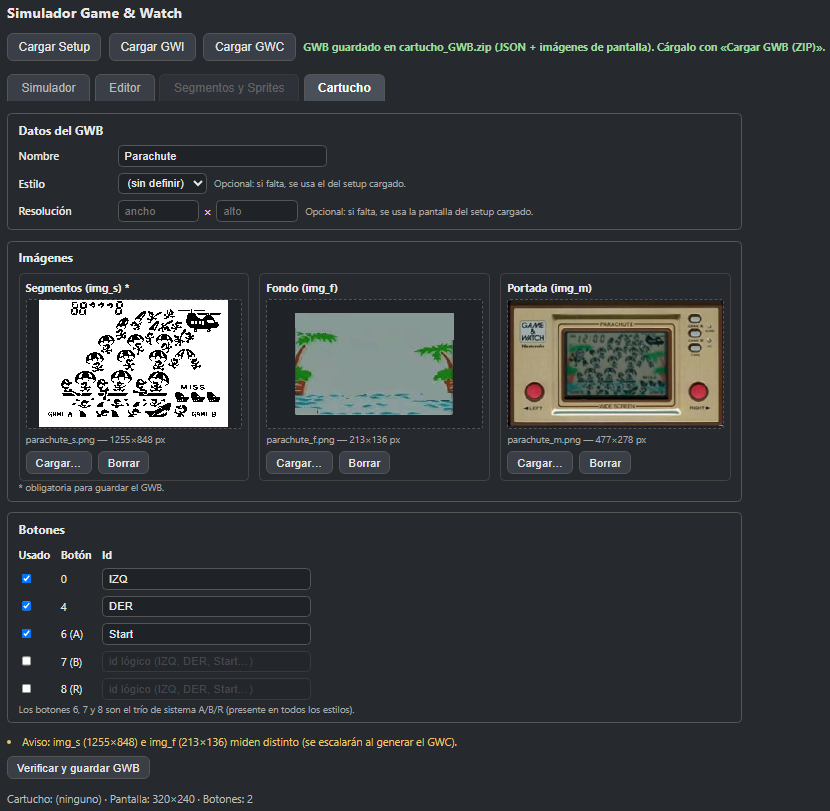
\includegraphics[width=0.60\linewidth]{imagenes/Propias/C05-I026}
	\caption[Pestaña de datos del Cartucho]{Pestaña de datos del Cartucho}
	\label{fig:c05-i026}
\end{figure}

\begin{itemize}
	\item Identidad: Con los campos para
	\begin{itemize}
		\item \texttt{nombre}: El que se desea dar al cartucho.
		\item \texttt{estilo}: El de los botones (2,4,5). 
		\item \texttt{resolucion}: La resolución que se usará en la pantalla.
		\item \texttt{codigoGWC}: Si existe el código del par (solo informativo y no editable).
	\end{itemize}
	
	\item Las tres imágenes del apartado \texttt{imagenes}, mostranso solo una miniatura, delante de cada uno el nombre img\_f, img\_s, img\_m como referencia rápida de cual es (redundante por que de arriba a abajo son siempre s f y m): 
	\begin{itemize}
		\item \textbf{img\_s}: Obligatoria. Imagen con todos los segmentos en blanco y negro. Cuando se cargue una imagen, se debe verificar explícitamente que solo se use blanco y negro puros\footnote{Se deja como ampliación poder cargar cualquier imagen y convertirla en Blanco y Negro}.
		\item \textbf{img\_f}: Opcional. La imagen del fondo, si no se define será fondo blanco.
		\item \textbf{img\_m}: Opcional. La miniatura que se usará en el selector de cartuchos.
	\end{itemize}
	\item Los botones declarados: tabla con \texttt{numero} e \texttt{id} de cada uno.
\end{itemize}

\subsection{La edición del cartucho cargado}
\label{sec:F5I10Edicion}

Con un GWB o un GWI cargado, la ficha pasa a ser manipulable: renombrar el cartucho,
cambiar los \texttt{id} de los botones y sustituir las imágenes por otro fichero 
local. Para ello se incluirán botones junto a cada imagen que permitan eliminarla 
y seleccionar un fichero png para cargarlo\footnote{al guardar los datos, los nombres 
de las imágenes serán siempre img\_f.png, img\_s.png, img\_m.png, por tanto no hace falta
incluir los nombres reales en la pantalla}, con estos límites:

\begin{itemize}
	\item \textbf{Sustituir img\_f o img\_m}: Directamente sin problemas.
	\item \textbf{Sustituir img\_s}: Ya que los sprites, segmentos y mapa proceden de esta imagen, se debe limitar el cambio:
	\begin{itemize}
		\item Si no hay segmentos en memoria: permitir el cambio sin más\footnote{Este caso solo se puede dar si no se ha cargado nada nunca, en cuanto se defina una imagen de segmentos o se cargue un cartucho ya se habrán creado los segmentos}.
		\item Si hay segmentos en memoria: se pide confirmar pues se eliminarán estos previamente a la carga, si se confirma se limpia la memoria completa en cuanto a  segmentos, imágenes, datos de base y la autoría. Solo permanecen los datos del cartucho que figuran en esta pestaña, así no hay posibilidad de mezclas de datos erróneas.
		\item Tras cargar la imagen, hay que forzar la re-extracción siempre (la pestaña Sprites y el mapa se recalculan).
	\end{itemize}
	
\end{itemize}

No serán editables ni \textbf{el estilo} ni \textbf{la resolución}: si difieren del setup de la máquina cargada, \texttt{validarGWB} ya lo bloquea al entrar; cambiarlo en caliente rompería la geometría de la pantalla, pero se deja como posible ampliación poder alterar estos valores, de forma que ya no sea necesario cargar un Setup previo a definir el cartucho.

El trío de botones estándar A/B/R no aparecerán en la lista de botones definibles en este momento, aunque será posible ampliar el sistema para su tratamiento.

Para editar los botones, al no ser crítico su modificación, se presenta la lista de los posibles según el estilo definido al cargar el setup, y se permite modificar los datos asociados.

\subsection{Crear un cartucho de cero}
\label{sec:F5I10Crear}

Cuando no hay cartucho cargado, la pestaña ofrece el asistente de
creación. No es un editor paralelo: es un generador del objeto
cartucho que termina entregándolo al flujo que ya existe, de modo que
un GWB creado de cero y uno cargado de disco son indistinguibles para
el resto del programa.

\begin{enumerate}
	\item Requiere el setup cargado: de él salen el \texttt{estilo} y
	los botones físicos entre los que se elige.
	\item El estilo no será editable, pues sale del setup cargado (se deja como ampliación poder hacerlo).
	\item Se seleccionan las imágenes desde ficheros locales: img\_s
	obligatoria, img\_f e img\_m opcionales.
	\item Se declaran los botones: se eligen entre los físicos del
	setup y se les da su \texttt{id} (A/B/R incluidos).
	\item Se construye el JSON en memoria, se valida con
	\texttt{validarGWB} (el mismo contrato de entrada) y se entrega al
	editor como cartucho en edición: extracción de sprites, mapa y
	botonera se comportan como tras una carga.
\end{enumerate}

\subsection{El guardado del GWB}
\label{sec:F5I10Guardado}

Guardar un cartucho en una carpeta de disco no es cosa que un
navegador sepa hacer sin más: no puede crear un directorio y escribir
ficheros dentro de forma general. La solución es usar el mismo sistema 
que utilizamos al guardar el GWI: un botón \textbf{Guardar GWB} en la 
ficha que genera \texttt{cartucho\_gwb.zip} con el JSON y las tres 
imágenes, con el mismo empaquetado (JSZip + \texttt{imagenBlob}) que ya existe.

La carga de ficheros ZIP ya está resuelta por la iteración anterior: el
núcleo de carga detecta la forma por el CONTENIDO
(\ref{sec:F5I9}), de modo que un GWB dentro de un fichero comprimido
sigue el camino ZIP → abrirZIP → recursión con el tipo esperado y 
carga como si fuera la carpeta. 

El único hueco es de entrada: el botón «Cargar GWB» usa hoy un selector 
de directorio (\texttt{webkitdirectory}), que no admite soltar un ZIP. 
\underline{En esta iteración} se añade pues la doble vía de entrada del 
GWB, carpeta o ZIP, desdoblando en dos botones, uno carga un directorio 
y otro carga un fichero; cuando la iteración que unifica la entrada del 
cartucho en un solo panel llegue (mejora futura de la \ref{sec:F5I9}), 
estos dos botones desaparecerán junto al resto de botones para cargar 
Cartuchos, permitiendo cargar indiferentemente ficheros sin comprimir, 
directorios o los ZIP comprimidos.

En cuanto a necesidad, el guardado del GWB no es imprescindible: el
GWB en memoria es la copia de trabajo y su salida natural es el GWI,
que ya es autónomo. Se incluye por completitud con el resto de
cartuchos: los tres formatos se pueden guardar, y así el cartucho
de base generado en el asistente sale del editor como fichero único,
sin depender de que el usuario monte la carpeta a mano.

\subsection{Qué cambia para el usuario}
\label{sec:F5I10Usuario}

Una pestaña nueva y dos capacidades que antes no existían: retocar
los datos de un cartucho (GWB o GWI) sin volver a su origen, y crear
un cartucho sin partir de una extracción. El GWC no cambia: se carga,
se juega y nada más.

\subsection{Mejora al guardar GWI/GWC}
\label{sec:F5I10Adicional}
Aunque no es del GWB, en esta iteración incluyo una pequeña mejora, 
la del par GWI+GWC: si se edita un GWI que lleva \texttt{codigoGWC} y 
se guarda, el GWC guardado deja de corresponderle. 

No es problemático, pero vamos a dar un aviso de forma explícita de que el par está
desequilibrado y conviene regenerar el GWC.

Además, añado en el GWI la resolución, de manera que tengamos toda la información necesaria en el cartucho intermedio siempre. De esta manera es posible diseñar una utilidad externa que convierta GWI en GWC sin tener que cargarlo en memoria (aunque esto no está previsto en este momento, puede ser una mejora).

\subsection{Pruebas de la iteración}
\label{sec:F5I10Pruebas}

\begin{itemize}
	\item La ficha refleja el cartucho cargado: nombre, estilo,
	tres miniaturas y tabla de botones, con GWB y con GWI.
	
	\item Editar nombre e ids y guardar produce un GWI cuyo JSON
	lleva los cambios; al recargarlo, la ficha los muestra.
	
	\item Sustituir img\_m y guardar: la imagen nueva viaja en el ZIP
	(cierre de la F5-I9) y el GWI recargado la muestra.
	
	\item Sustituir img\_s dispara el aviso y la re-extracción.
	
	\item El asistente produce un GWB válido: La función 
	\texttt{validarGWB} bloquea los casos malos (sin img\_s, 
	 sin estilo, etc.).
	
	\item Con un GWC cargado, la pestaña queda deshabilitada.
	
	\item Guardar GWB genera un ZIP que, recargado por la nueva vía
	(zip o carpeta), produce el mismo cartucho: misma ficha, mismos
	sprites, mismo juego.
\end{itemize}